\section{Background}
\label{cal:sec:background}

\subsection{Branch Target Buffer (BTB)}
BTB is used in the core front-end to identify whether a program counter (PC) corresponds to a branch instruction before the instruction itself is even fetched. As depicted in \Cref{cal:fig:conv-btb}, each BTB entry is composed of \textit{tag}, \textit{type}, and \textit{target} fields. BTB is indexed with the lower order PC bits and \textit{tag} field of the indexed entry is compared with the higher order PC bits. A match indicates that the PC belongs to a branch instruction. The \textit{type} field of the indexed BTB entry determines whether the branch is a call, return, conditional, or unconditional branch. The branch type determines whether the branch direction (\textit{taken/not taken}) needs to be predicted and where its target address is found. Call, return, and unconditional branches are always \textit{taken}, whereas for conditional branches, a direction predictor is used to predict their direction. If the branch is predicted to be taken, \textit{target} field in the BTB entry provides the address for the next instruction, except for returns. This is because a given function can be called from different call sites; as such, the return address is call-site dependent. Therefore, a return address stack (RAS) is typically employed to record return addresses at call-sites. On a function call, the call instruction pushes the return address to RAS, which is later popped by the corresponding return instruction.

\begin{figure}
\centering
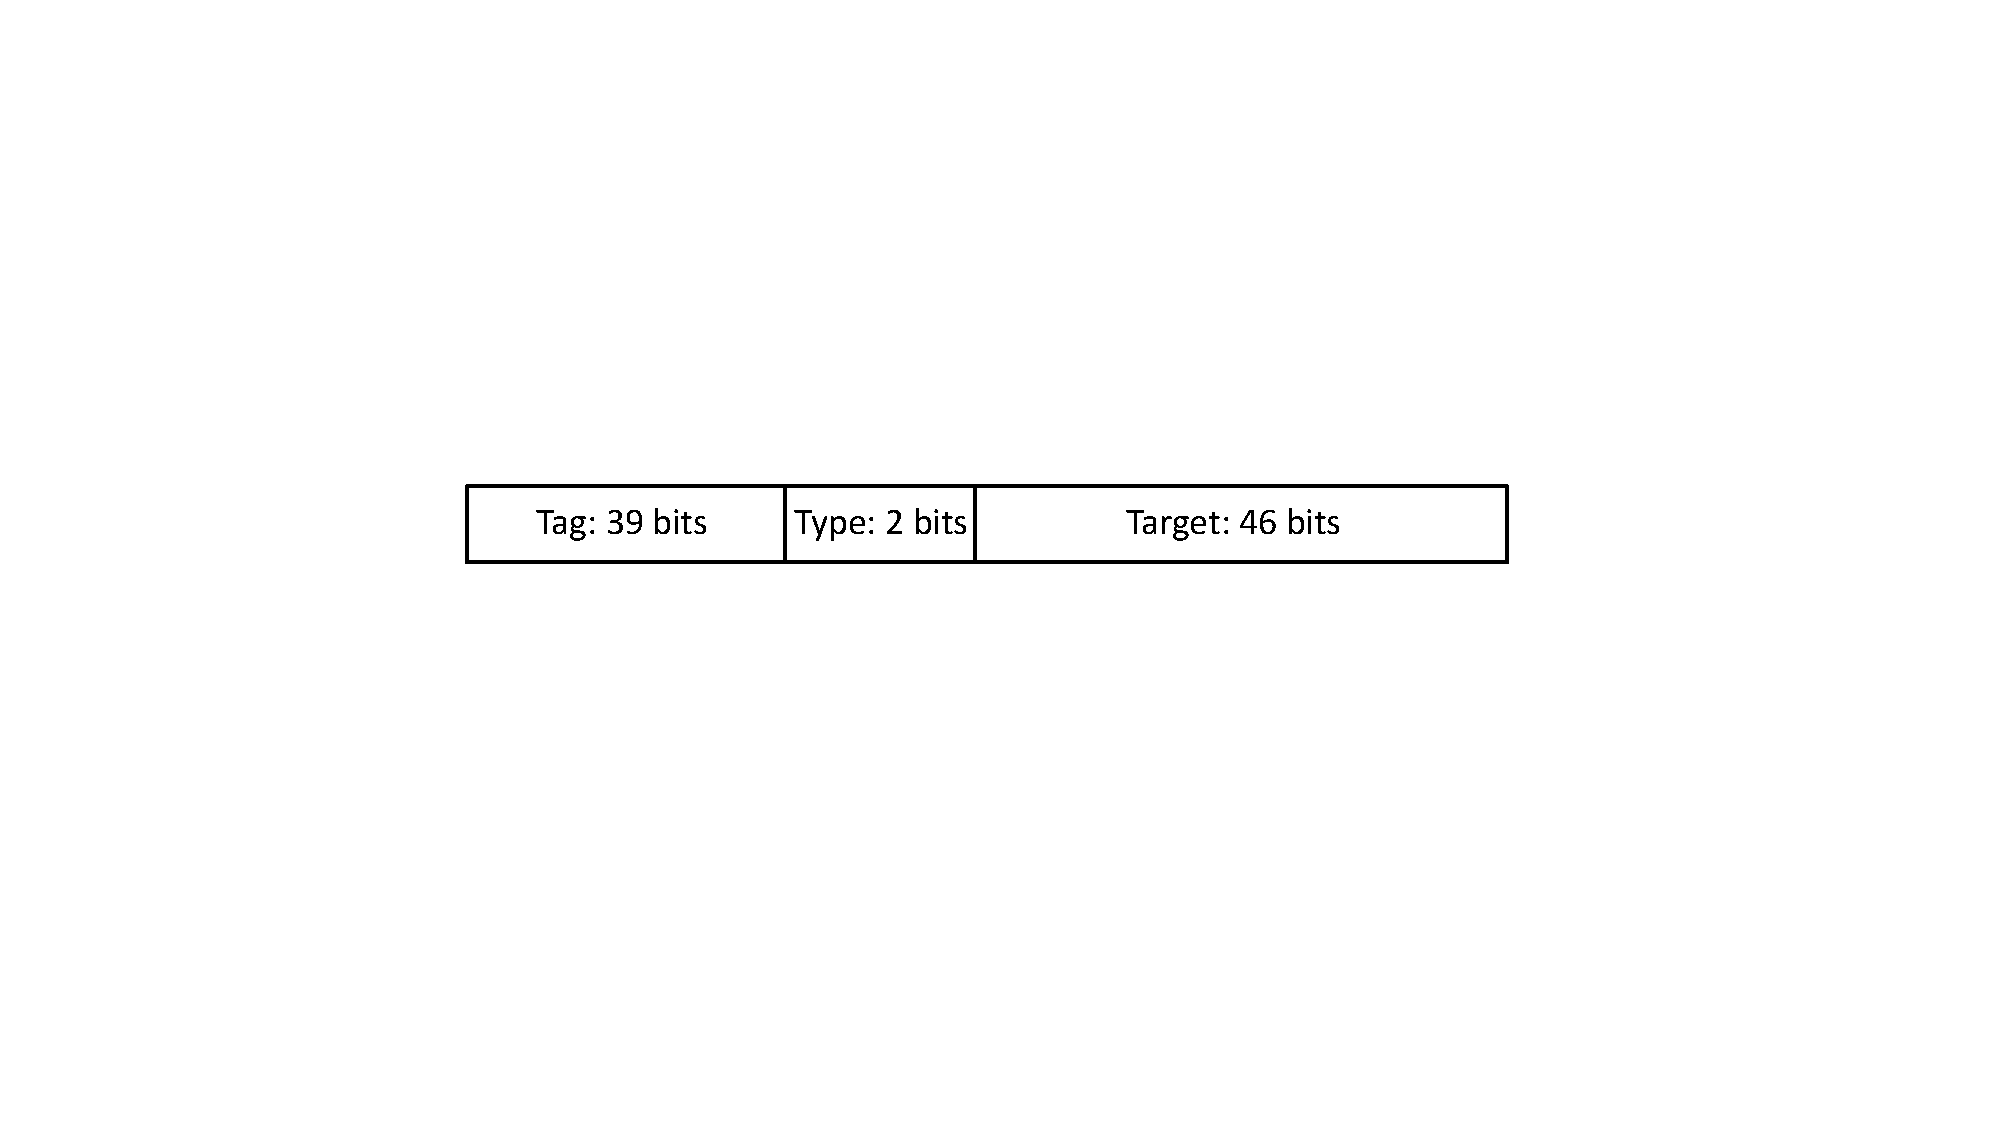
\includegraphics[width=0.8\columnwidth, trim=220 260 230 230, clip]{figures/baselineBTB1.pdf}
\caption {BTB entry composition in a conventional BTB. }
\label{cal:fig:conv-btb}
\end{figure}

\subsection{The cost of a BTB miss}
A BTB miss for a branch instruction means that the branch is undetected and the front-end continues to fetch instructions sequentially. Whether or not the sequential path is the correct one depends on the actual direction of the missed branch. Unless the missed branch is a conditional branch that is not taken, the sequential path is incorrect. When the wrong path is eventually detected by the core, all the instructions after the branch that missed in the BTB are flushed, fetch is redirected to the branch target and pipeline is filled with correct-path instructions. BTB misses are thus highly deleterious to performance as they result in a loss of tens of cycles of work and expose the pipeline fill latency. 


\subsection{BTB's role in instruction prefetching}
Fetch-directed instruction prefetchers are a class of powerful \liningfigures{L1-I} prefetchers that intrinsically rely on a BTB. 
These prefetchers are highly effective and, when coupled with a sufficiently large BTB, outperform the winner of the recently-concluded Instruction Prefetching Championship~\cite{ipc1}, as reported by Ishii et al.~\cite{rebase}. Variants of these prefetchers have been adopted in commercial products, for example in IBM z15~\cite{IBMz15HotChips}, ARM Neoverse N1~\cite{neoverse} etc.

\Cref{cal:fig:fdip} shows a canonical organization of a fetch-directed instruction prefetcher (FDIP)~\cite{fdip}. 
As originally proposed, FDIP decouples the branch-prediction unit and the fetch engine via the {\em fetch target queue (FTQ)}. This decoupling allows the branch prediction unit to run ahead of the fetch engine and discover prefetch candidates by predicting the control flow far into the future. With FDIP, each cycle, the branch prediction unit identifies and predicts branches to anticipate upcoming execution path and inserts corresponding instruction addresses into the FTQ. Consequently, the FTQ contains a stream of anticipated instruction addresses to be fetched by the core. The prefetch engine scans the FTQ to identify prefetch candidates and issue prefetch requests.

For FDIP to be effective, the BTB needs to accommodate the branch working set, otherwise frequent BTB misses will cause FDIP to prefetch the wrong path as FTQ will be filled with wrong path instruction addresses. This is one of the key reasons why commercial processors deploy massive BTBs, as also observed by~\cite{rebase}.


\begin{figure}
\centering
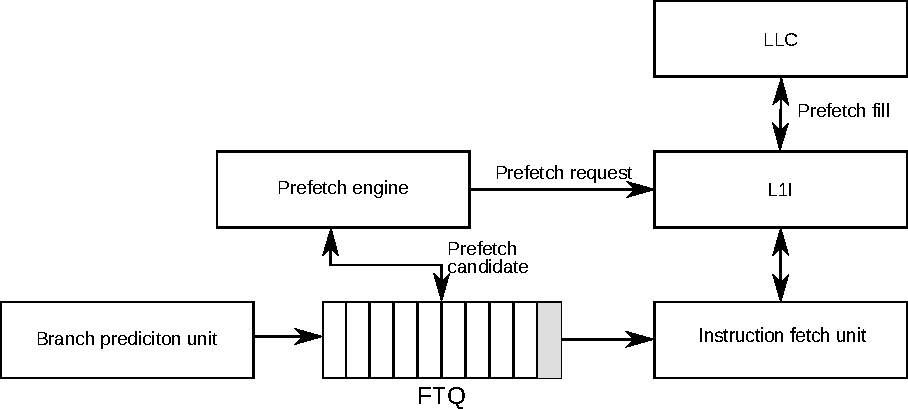
\includegraphics[width=.9\columnwidth, trim=0 0 0 0, clip]{figures/fdip1.pdf}
\caption{FDIP microarchitecture}
\vspace{-0.1in}
\label{cal:fig:fdip}
\end{figure}